%%%%%%%%%%%%%%%%%%%%%%%%%%%%%%%%%%%%%%%%%%%%%%%%%%%%%%%%%%%%%%%%%%%%
%%%           Vorlage für eine Ausarbeitung an der DHBW          %%%
%%%                                                              %%%
%%%      Bereiche die bearbeitet werden müssen werden durch      %%%
%%%      einen solchen Kommentarblock eingeleitet und enden      %%%
%%%      mit der nächsten Trennlinie.                            %%%
%%%                                                              %%%
%%%      In dieser Datei müssen folgende Bereiche bearbeitet     %%%
%%%      werden:                                                 %%%
%%%      - Angaben zur Arbeit                                    %%%
%%%      - EIGENE KAPITEL EINFÜGEN                               %%%
%%%                                                              %%%
%%%      Benötigte Seiten und Verzeichnisse können unter         %%%
%%%      "Einführung und Verzeichnisse" ein- bzw. auskommentiert %%%
%%%      werden.                                                 %%%
%%%                                                              %%%
%%%%%%%%%%%%%%%%%%%%%%%%%%%%%%%%%%%%%%%%%%%%%%%%%%%%%%%%%%%%%%%%%%%%

\documentclass[a4paper,12pt]{article}
\usepackage[left=2.5cm,right=2.5cm,top=2.5cm,bottom=2.5cm,includehead]{geometry}      % Einstellungen der Seitenränder
\usepackage[english, ngerman]{babel}                                                  % deutsche Silbentrennung
\usepackage[utf8]{inputenc}                                                           % Umlaute
\usepackage[official]{eurosym}                                                        % Euro Symbol
\usepackage[T1]{fontenc}													                                    % Umlaute auch richtig ausgeben
\usepackage{newtxtext,newtxmath}                                                      % Font = Times New Roman
\usepackage{hyperref}
\usepackage[nottoc]{tocbibind}
\usepackage{fancyhdr}
\usepackage{setspace}
\usepackage[backend=bibtex, citestyle=authoryear, bibstyle=authoryear]{biblatex}      % Bibliothek für Zitate
\usepackage{csquotes}                                                                 % Zusatzpacket für Zitate
\usepackage{amsmath}                                                                  % Zurücksetzen der Tabellen- und Abbildungsnummerierung je Sektion
\usepackage[labelfont=bf,aboveskip=1mm]{caption}                                      % Bild- und Tabellenunterschrift (fett)
\usepackage[bottom,multiple,hang,marginal]{footmisc}                                  % Fußnoten [Ausrichtung unten, Trennung durch Seperator bei mehreren Fußnoten]
\usepackage{graphicx}  
\graphicspath{{./images/}}                                                            % Grafiken
\usepackage[dvipsnames]{xcolor}                                                       % Farbige Buchstaben
\usepackage{wrapfig}                                                                  % Bilder in Text integrieren
\usepackage{enumitem}                                                                 % Befehl setlist (Zeilenabstand für itemize Umgebung auf 1 setzen)
\usepackage{listings}                                                                 % Quelltexte
\definecolor{commentgreen}{RGB}{87,166,74}                                            % Kommentar-Farbe für Quellcode
\lstset{numbers=left, numberstyle=\tiny, numbersep=8pt, frame=single, framexleftmargin=15pt, breaklines=true, commentstyle=\color{commentgreen}}
\usepackage{tabularx}                                                                 % Tabellen
\usepackage{multirow}                                                                 % Mehrzeilige Tabelleneinträge
\usepackage[addtotoc]{abstract}                                                       % Abstract
\usepackage[nohyperlinks, printonlyused, withpage]{acronym}                           % Abkürzungen
\usepackage{dirtree}                                                                  % Ordnerstruktur (z.B. für Anhang)

%%%%%%%%%%%%%%%%%%%%%%%%%%%%%%%%%%%%%%%%%%%%%%%%%%%%%%%%%%%%%%%%%%%%
%%%                      Angaben zur Arbeit                      %%%
%%%%%%%%%%%%%%%%%%%%%%%%%%%%%%%%%%%%%%%%%%%%%%%%%%%%%%%%%%%%%%%%%%%%
\def\vFirmenlogoPfad{}                  %% relativer Pfad Bsp.: images/Firmenlogo.png
\def\vDHBWLogoPfad{images/DHBW_logo.jpg}                          %% relativer Pfad Bsp.: images/DHBW_logo.jpg
\def\vUnterschrift{}                    %% Pfad zu Bild mit Unterschrift (für digitale Abgabe) Bsp.: images/Unterschrift.png

\def\vTitel{}                           %%
\def\vUntertitel{}                      %%
\def\vArbeitstyp{}                      %% Projektarbeit/Seminararbeit/Bachelorarbeit
\def\vArbeitsbezeichnung{}              %% T1000/T2000/T3000

\def\vAutor{}                           %% Vorname Nachname
\def\vMatrikelnummer{}                  %% 7-stellige Zahl
\def\vKursKuerzel{}                     %% Bsp.: TIT20
\def\vPhasenbezeichnung{}               %% Praxisphase/Theoriephase
\def\vStudienJahr{}                     %% erste/zweite/dritte
\def\vDHBWStandort{}                    %% Bsp.: Ravensburg
\def\vDHBWCampus{}                      %% Bsp.: Friedrichshafen
\def\vFakultaet{}                       %% Technik/Wirtschaft
\def\vStudiengang{}                     %% Informationstechnik/...

\def\vBetrieb{}                         %%
\def\vBearbeitungsort{}                 %%
\def\vAbteilung{}                       %%
\def\vBetreuer{}                        %% Vorname Nachname

\def\vAbgabedatum{\today}               %% DD. MONTH YYYY
\def\vBearbeitungszeitraum{}            %% DD.MM.YYYY - DD.MM.YYYY


%%%%%%%%%%%%%%%%%%%%%%%%% Eigene Kommandos %%%%%%%%%%%%%%%%%%%%%%%%%
% Definition von \gqq{} und \gq{}: Text in Anführungszeichen
\newcommand{\gqq}[1]{\glqq #1\grqq}
\newcommand{\gq}[1]{\glq #1\grq}
% Spezielle Hervorhebung von Schlüsselwörtern
\newcommand{\textOrdner}[1]{\texttt{#1}}
\newcommand{\textVariable}[1]{\texttt{#1}}
\newcommand{\textKlasse}[1]{\texttt{#1}}
\newcommand{\textFunktion}[1]{\texttt{#1}}


%%%%%%%%%%%%%%%%%%%% Zitatbibliothek einbinden %%%%%%%%%%%%%%%%%%%%%
\addbibresource{literatur/literatur.bib}
\addbibresource{literatur/tobias.bib}


%%%%%%%%%%%%%%%%%%%%%%%% PDF-Einstellungen %%%%%%%%%%%%%%%%%%%%%%%%%
\hypersetup{
  bookmarksopen=false,
	bookmarksnumbered=true,
	bookmarksopenlevel=0,
  pdftitle=\vTitel,
  pdfsubject=\vTitel,
  pdfauthor=\vAutor,
  pdfborder={0 0 0},
	pdfstartview=Fit,
  pdfpagelayout=SinglePage
}


%%%%%%%%%%%%%%%%%%%%%%%% Kopf- und Fußzeile %%%%%%%%%%%%%%%%%%%%%%%%
\pagestyle{fancy}
\setlength{\headheight}{15pt}
\fancyhf{}
\fancyhead[R]{\thepage}


%%%%%%%%%%%%%%%%%%%%%%%%%%%%%% Layout %%%%%%%%%%%%%%%%%%%%%%%%%%%%%%
\onehalfspacing
\setlist{noitemsep}

\addto\captionsngerman{
  \renewcommand{\figurename}{Abb.}
  \renewcommand{\tablename}{Tab.}
}
\numberwithin{table}{section}                               % Tabellennummerierung je Sektion zurücksetzen
\numberwithin{figure}{section}                              % Abbildungsnummerierung je Sektion zurücksetzen
\renewcommand{\thetable}{\arabic{section}.\arabic{table}}   % Tabellennummerierung mit Section
\renewcommand{\thefigure}{\arabic{section}.\arabic{figure}} % Abbildungsnummerierung mit Section
\renewcommand{\thefootnote}{\arabic{footnote}}              % Sektionsbezeichnung von Fußnoten entfernen

\renewcommand{\multfootsep}{, }                             % Mehrere Fußnoten durch ", " trennen


%%%%%%%%%%%%%%%%%%%%%%%%%%%%% Dokument %%%%%%%%%%%%%%%%%%%%%%%%%%%%%

\begin{document}


  %%%%%%%%%%%%%%%%%%% Einführung und Verzeichnisse %%%%%%%%%%%%%%%%%%%
  \pagenumbering{Roman}

  \begin{titlepage}
  \begin{minipage}{6in}
    \vspace*{-2cm}
    \centering
    \hspace{-2cm}
	\ifx\vFirmenlogoPfad\empty
	\else
    \raisebox{-0.5\height}{\includegraphics[height=4cm]{\vFirmenlogoPfad}}
  \fi
	\hfill
	\ifx\vDHBWLogoPfad\empty
	\else
   	\raisebox{-0.5\height}{\includegraphics[height=4cm]{\vDHBWLogoPfad}}
	\fi
  \end{minipage}
  \begin{center}
    \vspace*{0.5cm}
    \Huge\textbf{\vTitel}\\
		\ifx\vUntertitel\empty
		\else
			\Large\rm\vUntertitel\\
		\fi
		\vspace*{2cm}
		\Large\textbf{\vArbeitstyp}
		\ifx\vArbeitsbezeichnung\empty
		\else
			\textbf{\vArbeitsbezeichnung}
		\fi
		\\
		\normalsize
		über die \vPhasenbezeichnung\ des \vStudienJahr{n}\ Studienjahrs \\
		\vspace*{1cm}
		an der Fakultät für \vFakultaet\\
		im Studiengang \vStudiengang\\
		\vspace*{0.5cm}
		an der DHBW \vDHBWStandort\\
		\ifx\vDHBWCampus\empty
		\else
		Campus \vDHBWCampus\\
		\fi
		\vspace*{0.5cm}
		von\\
		\ifx\vAutor\empty
		\else
			\vAutor\\
		\fi
		\vspace*{1cm}
		\vAbgabedatum
		\vfill
  \end{center}
  \begin{tabular}{ll}
    Bearbeitungszeitraum:&\vBearbeitungszeitraum\\
    Matrikelnummer, Kurs:&\vMatrikelnummer, \vKursKuerzel\\
	  Dualer Partner:&\vBetrieb\\
	  Betreuer des Dualen Partners:&\vBetreuer\\
  \end{tabular}
\end{titlepage}
\newpage
\setcounter{page}{2}
  % \thispagestyle{empty}
\section*{\Huge{Sperrvermerk}}

\addcontentsline{toc}{section}{Sperrvermerk}
gemäß Ziffer 1.1.13 der Anlage 1 zu §§ 3, 4 und 5  der Studien- und Prüfungsordnung für die Bachelorstudiengänge im Studienbereich Technik der Dualen Hochschule Baden-Würt­tem­berg vom 29.09.2017.\\

\noindent \gqq{Der Inhalt dieser Arbeit darf weder als Ganzes noch in Auszügen Personen außerhalb des Prüfungsprozesses und des Evaluationsverfahrens zugänglich gemacht werden, sofern keine anders lautende Genehmigung vom Dualen Partner vorliegt.}

\vfill
\leavevmode
\newline
\parbox{6cm}{\strut\centering \vBearbeitungsort, \vAbgabedatum\hrule\strut\centering\footnotesize Ort, Datum} 
\hfill
\ifx\vUnterschrift\empty
\parbox{6cm}{\strut\hspace{1pt} \vAbteilung\hrule\strut\centering\footnotesize Abteilung, Unterschrift}
\else
\parbox{6cm}{\strut\hspace{1pt} \vAbteilung, \parbox[b]{3cm}{\vspace{-10cm}\includegraphics[width=3cm]{\vUnterschrift}}\hrule\strut\centering\footnotesize Abteilung, Unterschrift}
\fi
\vspace{1cm}

\newpage
  \thispagestyle{empty}
\section*{\Huge{Selbstständigkeitserklärung}}

\addcontentsline{toc}{section}{Selbstständigkeitserklärung}
gemäß Ziffer 1.1.13 der Anlage 1 zu §§ 3, 4 und 5  der Studien- und Prüfungsordnung für die Bachelorstudiengänge im Studienbereich Technik der Dualen Hochschule Baden-Würt­tem­berg vom 29.09.2017.

\noindent Ich versichere hiermit, dass ich meine Bachelorarbeit (bzw. Projektarbeit oder Studienarbeit bzw. Hausarbeit) mit dem Thema: 
\begin{center}
	\Large\textbf{\vTitel}
\end{center}
selbstständig verfasst und keine anderen als die angegebenen Quellen und Hilfsmittel benutzt habe. Ich versichere zudem, dass die eingereichte elektronische Fassung mit der gedruckten Fassung übereinstimmt.

\vfill
\leavevmode

\parbox{6cm}{\strut\centering \vBearbeitungsort, \vAbgabedatum\hrule\strut\centering\footnotesize Ort, Datum} 
\hfill
\ifx\vUnterschrift\empty
\parbox{6cm}{\strut\hspace{1pt} \vAbteilung, \hrule\strut\centering\footnotesize Tobias Götz}
\else
\parbox{6cm}{\strut\hspace{1pt} \vAbteilung, \parbox[b]{3cm}{\vspace{-10cm}\includegraphics[width=3cm]{\vUnterschrift}}\hrule\strut\centering\footnotesize Tobias Götz}
\fi
\vspace{1cm}

\parbox{6cm}{\strut\centering \vBearbeitungsort, \vAbgabedatum\hrule\strut\centering\footnotesize Ort, Datum}
\hfill
\ifx\vUnterschriftKempter\empty
\parbox{6cm}{\strut\hspace{1pt} \vAbteilung, \hrule\strut\centering\footnotesize Noel Kempter}
\else
\parbox{6cm}{\strut\hspace{1pt} \vAbteilung, \parbox[b]{3cm}{\vspace{-10cm}\includegraphics[width=3cm]{\vUnterschriftKempter}}\hrule\strut\centering\footnotesize Noel Kempter}
\fi
\vspace{1cm}

\parbox{6cm}{\strut\centering \vBearbeitungsort, \vAbgabedatum\hrule\strut\centering\footnotesize Ort, Datum}
\hfill
\ifx\vUnterschriftKuest\empty
\parbox{6cm}{\strut\hspace{1pt} \vAbteilung, \hrule\strut\centering\footnotesize Philipp Küst}
\else
\parbox{6cm}{\strut\hspace{1pt} \vAbteilung, \parbox[b]{3cm}{\vspace{-10cm}\includegraphics[width=3cm]{\vUnterschriftKuest}}\hrule\strut\centering\footnotesize Philipp Küst}
\fi
\vspace{1cm}

\newpage
  \phantomsection
\newenvironment{keywords}{
	\begin{flushleft}
	\small	
	\textbf{
		\iflanguage{ngerman}{Schlüsselwörter}{\iflanguage{english}{Keywords}{}}
	}
}{\end{flushleft}}

% Deutsche Zusammenfassung
\begin{abstract}
	
\end{abstract}

% Schlüsselwörter Deutsch
\begin{keywords}
	
\end{keywords}


\selectlanguage{english}
% Englisches Abstract
\begin{abstract}

\end{abstract}

% Schlüsselwörter Englisch
\begin{keywords}

\end{keywords}


\selectlanguage{ngerman}
\newpage
  \tableofcontents
\newpage
  \section*{Abkürzungsverzeichnis}
\addcontentsline{toc}{section}{Abkürzungsverzeichnis}
\begin{acronym}
  \acro{DHBW}[DHBW]{Duale Hochschule Ba\-den-\-Würt\-tem\-berg}
  \acroplural{DHBW}[DHBW]{Dualen Hochschule Ba\-den-\-Würt\-tem\-berg}
\end{acronym}
\newpage
  \listoffigures
\newpage
  \listoftables
\newpage
  \lstlistoflistings
\addcontentsline{toc}{section}{Listings}
\newpage
  % \section*{Vorwort}
\addcontentsline{toc}{section}{Vorwort}
\newpage


  %%%%%%%%%%%%%%%%%%%%%%%%%%%%% Kapitel %%%%%%%%%%%%%%%%%%%%%%%%%%%%%%
  \pagestyle{fancy}
  \fancyhead[L]{\nouppercase{\rightmark}}    % Abschnittsname im Header
  \pagenumbering{arabic}

  %%%%%%%%%%%%%%%%%%%%%%%%%%%%%%%%%%%%%%%%%%%%%%%%%%%%%%%%%%%%%%%%%%%%
  %%%%                   EIGENE KAPITEL EINFÜGEN                  %%%%
  %%%%%%%%%%%%%%%%%%%%%%%%%%%%%%%%%%%%%%%%%%%%%%%%%%%%%%%%%%%%%%%%%%%%
  \section{Einleitung}
\subsection{Aufgabenstellung}
Im Rahmen dieser Hausarbeit soll eine Anforderungsanalyse für ein Softwareprojekt durchgeführt werden.
Dabei soll ein Video-on-Demand System entwickelt werden, welches es ermöglicht, Videos über das Internet anzusehen.
Dies soll in Anlehnung an die Webseite \url{https://www.primevideo.com} erfolgen.
Einschränkend ist dabei zu erwähnen, dass ausschließlich aktuelle Kinofilme angeboten werden sollen.
Ältere Filme oder Serien sollen somit nicht vom System angeboten werden.

\subsection{Aufbau der Arbeit}
Dieses Dokument ist in zwei Teile aufgeteilt.
Im ersten Teil wird auf die wissenschaftliche Herangehensweise an die Anforderungsanalyse eingegangen.
Hierzu werden die einzelnen Aspekte einer Anforderungsanalyse beschrieben und die einzelnen Methoden, welche in der Anforderungsanalyse verwendet werden, erklärt.
Dies wird mit wissenschaftlichen Quellen untermauert, um die allgemeine Qualität dieser Anforderungsanalyse zu gewährleisten.

Der zweite Teil beschreibt die praktische Umsetzung der Anforderungsanalyse des Video-on-Demand Systems.
Auf Basis der in Teil 1 beschriebenen Methoden wird Schritt für Schritt erklärt, wie die Ergebnisse der Anforderungsanalyse entstanden sind.
Der Fokus hierbei liegt auf den erarbeiteten Anforderungen, auf welche im Text zwar eingegangen wird, jedoch nicht im Detail.
Der gesamte Anforderungskatalog befindet sich im Anhang, um eine bessere Übersichtlichkeit zu gewährleisten.
Auf diese Weise kann der Leser die Anforderungen nachlesen, ohne den Text zu stören.

  \subsection{Widersprüche der Anforderungen}\label{subsec:widersprueche}
\gqq{Zwei Anforderungen widersprechen einander, wenn sie nicht durch dieselbe technische Lösung umgesetzt werden können.}\autocite[][S.233]{Herrmann.2022}
So definiert Herrmann Widersprüche.
Widersprüche können sich aus unterschiedlichen Gründen ergeben.
So können Widersprüche zum Beispiel in Bezug auf die Qualität, die Kosten oder die Zeit entstehen.

In diesem Kapitel wird erläutert, wie Widersprüche erkannt, analysiert und gelöst werden können.

\subsubsection{Erkennen von Widersprüchen}\label{subsubsec:erkennung}
Bevor Widersprüche gelöst werden können, müssen sie zuerst erkannt werden.
Es gibt verschiedene Indikatoren, die auf Widersprüche hinweisen können.
\begin{itemize}
    \item Bisher getroffene Aussagen werden ignoriert oder verändert, so als wären diese nie getroffen worden.
    \item Blindes Zustimmen zu oder Ablehnen von Aussagen anderer.
    \item Pedanterie
    \item Aussagen anderer werden bis ins kleinste Detail hinterfragt.
    \item Informationen oder Informationsdetails werden verheimlicht.
    \item Man lässt sich nur auf vage Aussagen ein, mit der Aufforderung an andere, diese zu detaillieren.
\end{itemize}~\autocite[vgl.][S.43]{OliverCreighton.2012}

\subsubsection{Analyse von Widersprüchen}\label{subsubsec:analyse}
Bevor Widersprüche gelöst werden können, müssen diese analysiert werden.
Dazu werden die Ursachen für den Widerspruch ermittelt.
Auch können Widersprüche in verschiedene Kategorien eingeteilt werden.

Hierbei wird zwischen drei Arten von Widersprüchen unterschieden:
\begin{itemize}
    \item Inkonsistenz
    \item Anforderungskonflikte
    \item Machbarkeitskonflikte
\end{itemize}~\autocite[vgl.][S.235f]{OliverCreighton.2012}

\paragraph{Inkonsistenz}
Ein Anforderungswiderspruch vom Typ Inkonsistenz bezieht sich auf Inkonsistenzen zwischen verschiedenen Anforderungen,
die sich auf den Problemraum beziehen.
Dies können beispielsweise Inkonsistenzen in der Terminologie, unklare Formulierungen,
fehlende Informationen, falsche Inhalte oder mehrdeutige Aussagen sein.
Das bedeutet, dass die Anforderungen untereinander in Konflikt stehen, aber keine technischen Probleme aufweisen.
Inkonsistenzen können durch Anforderungsreviews entdeckt werden, bei denen Anforderungen thematisch gruppiert werden,
um festzustellen, ob sie widersprüchliche Aussagen enthalten.
Inkonsistenzen werden durch eine Entscheidung im Problemraum gelöst,
zum Beispiel durch eine Klärung der Terminologie oder durch eine Überarbeitung der Formulierungen.\autocite[vgl.][S.235]{Herrmann.2022}

\paragraph{Anforderungskonflikt}
Ein Anforderungskonflikt ist ein Widerspruchstyp,
bei dem zwei oder mehr Anforderungen an ein System oder einen Prozess miteinander in Konflikt stehen.
Das bedeutet, dass es nicht möglich ist, alle Anforderungen gleichzeitig zu erfüllen,
da sie sich gegenseitig widersprechen oder unvereinbar sind.
Anforderungen können aus verschiedenen Quellen stammen, wie zum Beispiel Kundenanforderungen,
gesetzliche Vorschriften oder technische Einschränkungen.
Ein Beispiel für einen Anforderungskonflikt könnte sein,
dass ein System sowohl extrem sicher als auch sehr einfach zu bedienen sein soll.
Diese beiden Anforderungen sind miteinander in Konflikt,
da zusätzliche Sicherheitsmaßnahmen in der Regel die Benutzerfreundlichkeit beeinträchtigen können.
Anforderungskonflikte können in der Planungs- und Entwicklungsphase eines Systems oder Prozesses auftreten
und erfordern oft eine sorgfältige Abwägung und Priorisierung der verschiedenen Anforderungen.\autocite[vgl.][S.235f]{Herrmann.2022}

\paragraph{Machbarkeitskonflikt}
Ein Machbarkeitskonflikt ist ein Widerspruchstyp,
bei dem zwei oder mehr Anforderungen an ein System oder einen Prozess in Konflikt geraten,
da sie nicht gleichzeitig erfüllt werden können,
ohne dass es zu einem Verlust von Effizienz, Qualität oder Sicherheit kommt.
In diesem Konflikt geht es darum, dass die Anforderungen gegenseitig die Machbarkeit beeinträchtigen.

Ein Beispiel dafür ist der Konflikt zwischen der Notwendigkeit, ein System sehr sicher zu machen,
und der Notwendigkeit, es sehr effizient zu gestalten.
Eine sehr sichere Methode kann beispielsweise zusätzliche Überprüfungen und Genehmigungen erfordern,
was zu längeren Wartezeiten führt und somit die Effizienz beeinträchtigen kann.
Umgekehrt kann eine sehr effiziente Methode möglicherweise notwendige Sicherheitschecks vernachlässigen
und damit die Sicherheit des Systems beeinträchtigen.\autocite[vgl.][S.236]{Herrmann.2022}

\subsubsection{Lösen von Widersprüchen}\label{subsubsec:loesen}
Alle Widersprüche auf einmal zu lösen, ist nicht möglich,
denn durch das Lösen eines Widerspruchs kann ein anderer entstehen.
Daher ist es wichtig, die Widersprüche in einer bestimmten Reihenfolge zu lösen.
Hierbei wird sich zuerst auf Widersprüche auf höchster und abstraktester Ebene konzentriert,
denn diese haben die größte Auswirkung auf das System und arbeitet sich dann nach unten vor.

\paragraph{Reihenfolge der Widerspruchsauflösung}
\begin{enumerate}
    \item Durch ein Anforderungsreview Inkonsistenzen und Anforderungskonflikte erkennen.
    \item Inkonsistenzen im Problemraum lösen.
    \item Konflikte zwischen Stakeholder lösen.
    \item Anforderungskonflikte und Machbarkeitskonflikte im Lösungsraum lösen.
    Hier kommen zum Beispiel Nutzwertanalyse oder Quality Function Deployment zum Einsatz.
\end{enumerate}\autocite[vgl.][S.237f]{Herrmann.2022}

\subsubsection{Konflikttypen}
Um Konflikte besser lösen zu können, ist es wichtig, die verschiedenen Konflikttypen zu kennen.
Diese sind:
\begin{itemize}
    \item Sachkonflikt
    \item Datenkonflikt
    \item Interessenkonflikt
    \item Wertekonflikt
    \item Beziehungskonflikt
    \item Struktureller Konflikt
\end{itemize}\autocite[vgl.][S.137]{Pohl.2021}

\paragraph{Sachkonflikt}
\gqq{
    Ein Sachkonflikt zwischen zwei oder mehr Stakeholdern ist durch einen Mangel an Informationen
    oder durch Fehlinformation gekennzeichnet.
}~\autocite[][S.138]{Pohl.2021}

\paragraph{Datenkonflikt}
\gqq{
    Eine spezielle Ausprägung des Sachkonflikts ist der Datenkonflikt(auch Benennungskonflikt).
    Bei einem Datenkonflikt verstehen die beteiligten Stakeholder unterschiedliche Dinge unter einem Bezeichner
}~\autocite[][S.138]{Pohl.2021}

\paragraph{Interessenkonflikt}
\gqq{
    Ein Interessenkonflikt zwischen zwei oder mehr Stakeholdern ist durch
    subjektiv oder objektiv verschiedene Interessen oder Ziele der Stakeholder gekennzeichne
}~\autocite[][S.138]{Pohl.2021}

\paragraph{Wertekonflikt}
\gqq{
    Ein Wertekonflikt ist durch verschiedene Kriterien (z. B. kulturelle Unterschiede, persönliche Ideale)
    von Stakeholdern zur Bewertung von Sachverhalten gekennzeichnet
}~\autocite[][S.138]{Pohl.2021}

\paragraph{Beziehungskonflikt}
\gqq{
    Ein Beziehungskonflikt ist durch starke Emotionen, stereotype Beziehungskonzepte, schlechte Kommunikation
    oder negatives zwischenmenschliches Verhalten von Stakeholdern untereinander
    (z. B. Missachtung, Beleidigung) gekennzeichnet.
}~\autocite[][S.138]{Pohl.2021}

\paragraph{Struktureller Konflikt}
\gqq{
    KonfliktEin struktureller Konflikt ist durch ungleiche Macht- und Autoritätsverhältnisse
    zwischen Stakeholdern gekennzeichnet.
}~\autocite[][S.138]{Pohl.2021}

\subsubsection{Konsolidierungstechniken}
Es gibt verschiedene Konfliktlösungstechniken,
die bei der Konsolidierung von Widersprüchen helfen können.
Die Lösungstechniken werden in der Regel in der genannten Reihenfolge angewendet.
Diese sind:
\begin{enumerate}
    \item Einigung
    \item Kompromiss
    \item Abstimmung
    \item Variantenbildung
    \item Ober-sticht-Unter
\end{enumerate}\autocite[vgl.][S.139]{Pohl.2021}

\paragraph{Einigung}
\gqq{
    Bei der Konfliktlösungstechnik Einigung handeln die Konfliktparteien eine Lösung des Konflikts aus.
    Die Konfliktparteien tauschen Informationen, Argumente und Meinungen aus
    und versuchen sich gegenseitig im Dialog von der Richtigkeit des eigenen Standpunkts zu überzeugen
    und sich so auf eine Lösungsalternative des Konflikts zu einigen.
}~\autocite[][S.139]{Pohl.2021}

\paragraph{Kompromiss}
\gqq{
    Bei der Konfliktlösungstechnik Kompromiss versuchen die Konfliktparteien im Rahmen einer Diskussion
    einen Kompromiss zwischen den verfügbaren Lösungsalternativen zu finden.
    Im Unterschied zur Einigung besteht ein Kompromiss aus einer Kombination
    von Teilen der verfügbaren Lösungsalternativen.
    Ebenso kann ein Kompromiss auch darin bestehen,
    dass alle Lösungsalternativen verworfen werden und eine vollkommen neue und kreative Lösung entwickelt wird.
}~\autocite[][S.140]{Pohl.2021}

\paragraph{Abstimmung}
\gqq{
    Bei der Konfliktlösungstechnik Abstimmung wird die Lösung eines Konflikts durch eine Abstimmung erzielt.
    Die zur Wahl stehenden Alternativen werden den relevanten Stakeholdern zur Abstimmung vorgelegt.
    Jeder Stakeholder gibt seine Stimme einer der Alternativen.
    Die Alternative mit den meisten Stimmen wird als Konfliktlösung festgehalten.
}~\autocite[][S.140]{Pohl.2021}

\paragraph{Variantenbildung}
\gqq{
    Bei der Konfliktlösungstechnik Variantenbildung wird das System so gestaltet,
    dass durch Variantenauswahl oder Parametrierung verschiedene Systemvarianten realisiert
    oder Auswahlmöglichkeiten bei variablen Systemmerkmalen ermöglicht werden,
    wodurch das System unterschiedlichen, im Konflikt stehenden Interessen von Stakeholdern genügen kann.
}~\autocite[][S.140]{Pohl.2021}

\paragraph{Ober-sticht-Unter}
\gqq{
    Bei der Konfliktlösungstechnik Ober-sticht-Unter wird ein Konflikt anhand der Hierarchie
    der Konfliktparteien entschieden, d. h., die Konfliktpartei mit dem höheren organisatorischen Rang
    gewinnt den Konflikt.
    Wenn beide Konfliktparteien den gleichen organisatorischen Rang einnehmen,
    wird der Konflikt durch eine übergeordnete Instanz (z. B. einen Vorgesetzten) entschieden.
    Diese Konfliktlösungstechnik ist nur dann empfehlenswert,
    wenn andere Lösungstechniken zu keiner Lösung geführt haben (z. B. kein Kompromiss gefunden werden konnte)
    oder aus Ressourcengründen nicht anwendbar sind.
}


In Abbildung~\nameref{fig:konsolidierungstechniken} ist eine Übersicht über die Konsolidierungstechniken dargestellt,
und wann es sinnvoll ist diese anzuwenden.
\begin{figure}[ht]
    \centering
    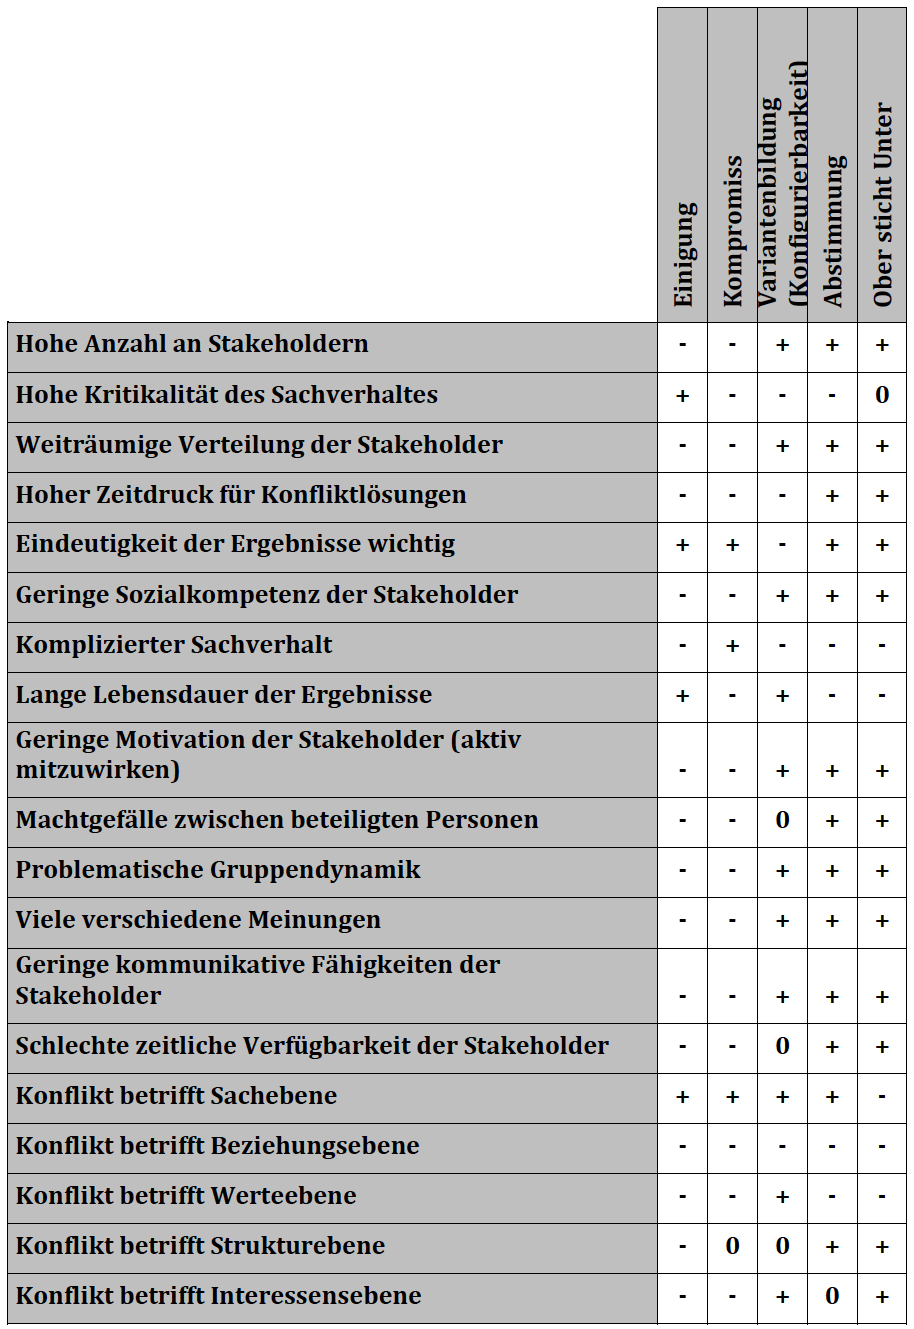
\includegraphics[width=0.8\textwidth]{images/KonsolidierungstechnikenTabelle}
    \caption{Konsolidierungstechniken}
    \label{fig:konsolidierungstechniken}
\end{figure}~\autocite[Abbildung 5][S.45]{OliverCreighton.2012}

  %%%%%%%%%%%%%%%%%%%%%%% Literaturverzeichnis %%%%%%%%%%%%%%%%%%%%%%%
  \phantomsection
\addcontentsline{toc}{section}{Literatur}
\printbibliography
\newpage


  %%%%%%%%%%%%%%%%%%%%%%%%%%%%%% Anhang %%%%%%%%%%%%%%%%%%%%%%%%%%%%%%
  \renewcommand{\thetable}{\Alph{section}.\arabic{table}}
  \renewcommand{\thefigure}{\Alph{section}.\arabic{figure}}
  \renewcommand{\thelstlisting}{\Alph{section}.\arabic{lstlisting}}
  \pagenumbering{Alph}

  \begin{appendix}
  \section{Anhang}
\end{appendix}
\end{document}